\chapter{Frontend Implementation and UI/UX Design System}

\section{Introduction}
StayMart's user interface is engineered to deliver an authentic, high-trust accommodation and classifieds marketplace specifically tailored for students in Uttarakhand. Traditional classifieds suffer from visual clutter and misleading photos, while heavy Single-Page Applications (SPAs) impose large JavaScript payloads that struggle on congested campus cellular networks. StayMart utilizes native HTML5, modern CSS3 custom properties, and modular ES6 JavaScript without bundler overhead, achieving sub-45 KB payloads and sub-second rendering.

\section{Design Philosophy and Visual Design System}
Rather than adopting generic dark-mode templates, StayMart establishes a high-trust commercial light aesthetic grounded in Uttarakhand's academic geography (Figure \ref{fig:landing_page_ui}).

\begin{figure}[htbp]
    \centering
    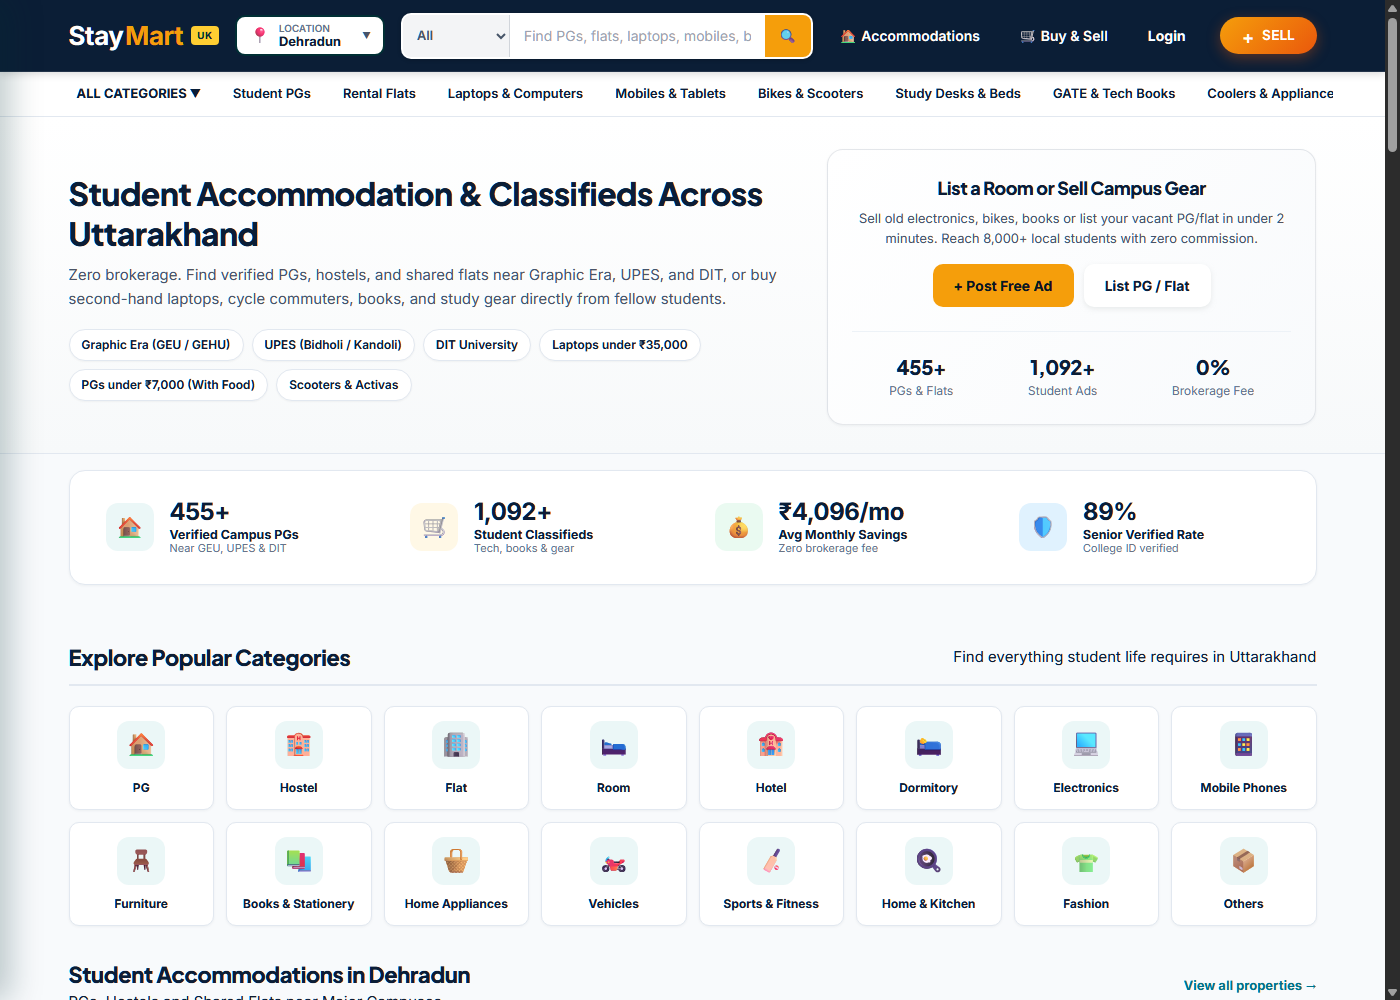
\includegraphics[width=0.92\textwidth]{screenshots/landing_page.png}
    \caption{StayMart Modern Landing Interface Featuring Alpine Navy Navigation, Refined Campus Chips, and Real-Time Marketplace Metrics}
    \label{fig:landing_page_ui}
\end{figure}

The visual system is governed by: (1) \textit{Subject-Matter Grounding}: proximity chips (``400m from GEHU Gate 2''), verified roommate badges, and student gear categories; (2) \textit{High-Contrast Commercial Dignity}: pearl white canvas (\texttt{\#f8fafc}), white cards (\texttt{\#ffffff}), and slate borders (\texttt{\#e2e8f0}); and (3) \textit{Structured Elevation}: multi-layer soft shadows without distracting glassmorphism.

\subsection{Color Palette and Design Tokens}
Declared in \texttt{:root} in \texttt{frontend/css/global.css}, key tokens define semantic brand identity:

\begin{lstlisting}[language=HTML, caption={Core Design Tokens in frontend/css/global.css}, label={lst:design_tokens}]
:root {
  --header-bg: #0b1e36;          /* Deep Himalayan Alpine Navy */
  --header-text: #ffffff;
  --amazon-amber: #f59e0b;        /* Radiant Conversion Accent */
  --success: #10b981;             /* Emerald Mint Verified */
  --bg-page: #f8fafc;             /* Crisp Pearl White Canvas */
  --bg-card: #ffffff;
  --text-primary: #0b1e36;        /* High-contrast deep slate */
  --text-secondary: #475569;      /* Slate subtitles (WCAG AAA) */
  --border: #e2e8f0;              /* Delicate slate borders */
  --shadow-md: 0 4px 16px -2px rgba(11, 30, 54, 0.08);
  --font: 'Inter', -apple-system, sans-serif;
  --font-display: 'Plus Jakarta Sans', var(--font);
}
\end{lstlisting}

Typography combines geometric display headings in \textbf{Plus Jakarta Sans} with high-legibility body prose in \textbf{Inter}.

\section{Modular Client-Side JavaScript Architecture}
Frontend functionality is organized into modular scripts in \texttt{frontend/js/}:
\begin{itemize}
    \item \textbf{\texttt{api.js}:} Manages dynamic base URL detection, automatic JWT token extraction/injection, and standardized \texttt{ApiResponse<T>} payload unwrapping.
    \item \textbf{\texttt{auth.js}:} Validates session state via \texttt{GET /api/users/me}, protects private routes, enforces admin guard roles, and coordinates header UI hydration.
    \item \textbf{\texttt{stats.js} \& \texttt{charts.js}:} Powers animated counters via \texttt{IntersectionObserver}, dual savings calculators, and Chart.js rental distributions.
    \item \textbf{\texttt{utils.js} \& \texttt{behavior.js}:} Provides XSS sanitization via \texttt{escapeHtml()}, Indian Rupee currency formatting, and non-blocking telemetry event tracking.
\end{itemize}

\section{Public Portals and User Flows}

\subsection{Authentication and Onboarding Portals}
Dedicated authentication portals (\texttt{login.html} and \texttt{register.html}) feature empty form states with browser autofill disabled, interactive password visibility toggles, and real-time email validation (Figure \ref{fig:auth_screens}).

\begin{figure}[htbp]
    \centering
    \begin{subfigure}[b]{0.48\textwidth}
        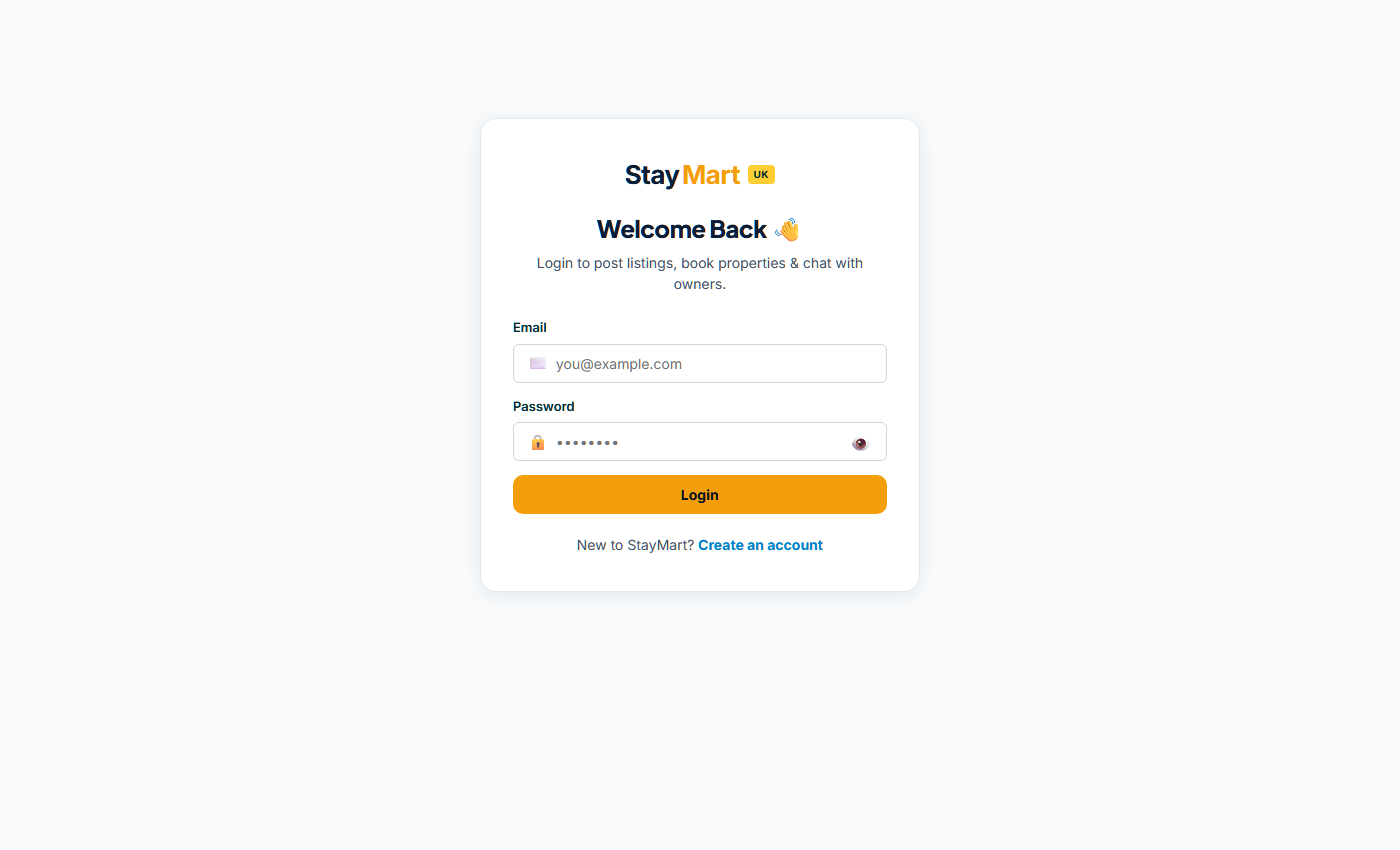
\includegraphics[width=\textwidth]{screenshots/login_page.png}
        \caption{Clean Student & Host Login Interface}
    \end{subfigure}
    \hfill
    \begin{subfigure}[b]{0.48\textwidth}
        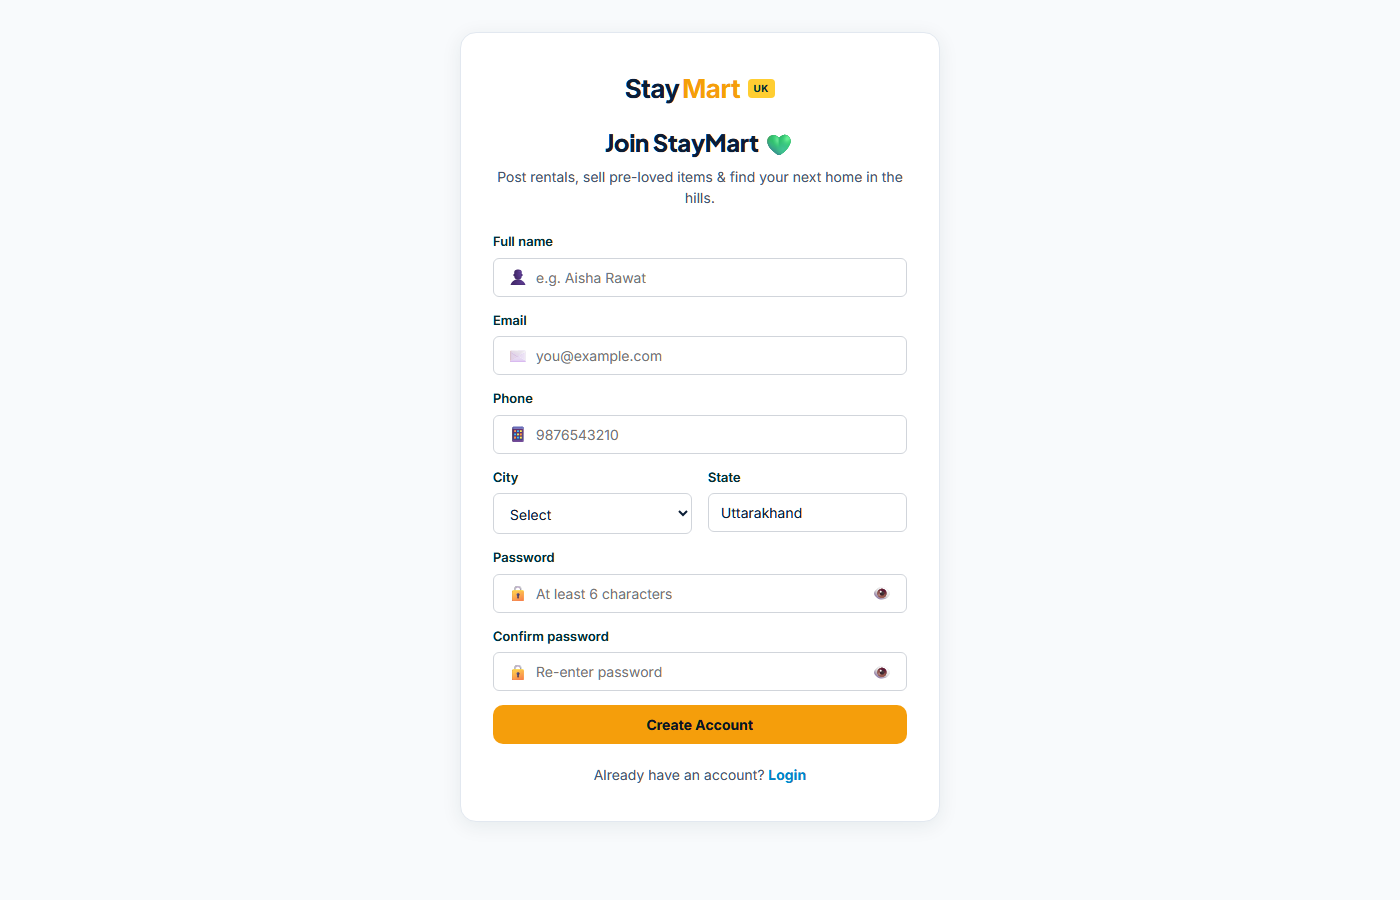
\includegraphics[width=\textwidth]{screenshots/register_page.png}
        \caption{Student Registration with Verification}
    \end{subfigure}
    \caption{Authentication Portals Featuring Clean Credential Inputs and Password Visibility Toggles}
    \label{fig:auth_screens}
\end{figure}

\subsection{Faceted Accommodation and Product Search Portals}
The search portals (\texttt{search-properties.html} and \texttt{search-products.html}) provide multi-attribute faceted filtering (Figure \ref{fig:search_screens}).

\begin{figure}[htbp]
    \centering
    \begin{subfigure}[b]{0.48\textwidth}
        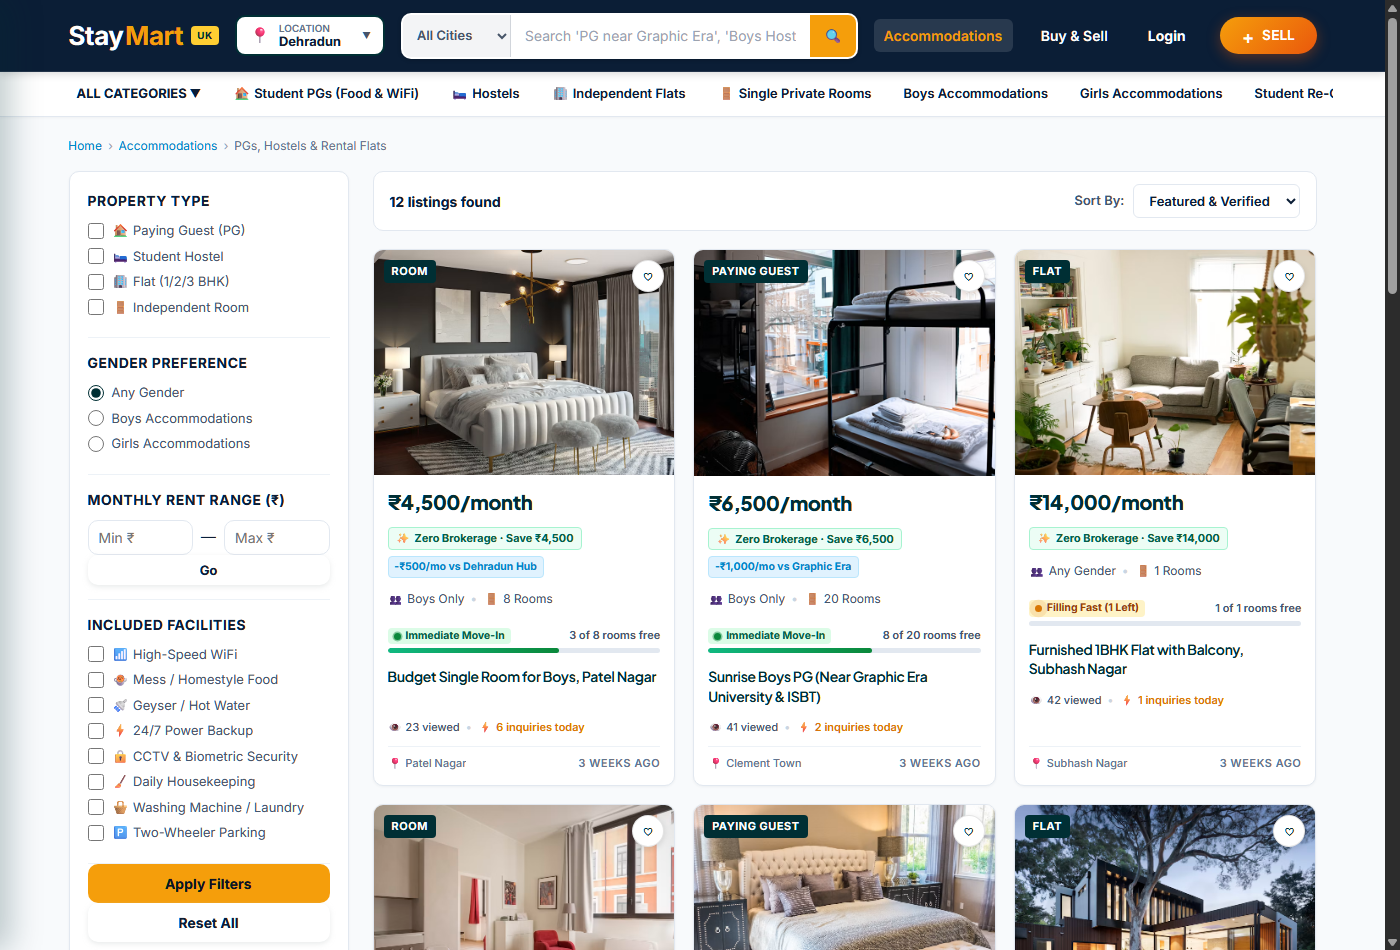
\includegraphics[width=\textwidth]{screenshots/search_properties.png}
        \caption{Property Search with Amenities Filter}
    \end{subfigure}
    \hfill
    \begin{subfigure}[b]{0.48\textwidth}
        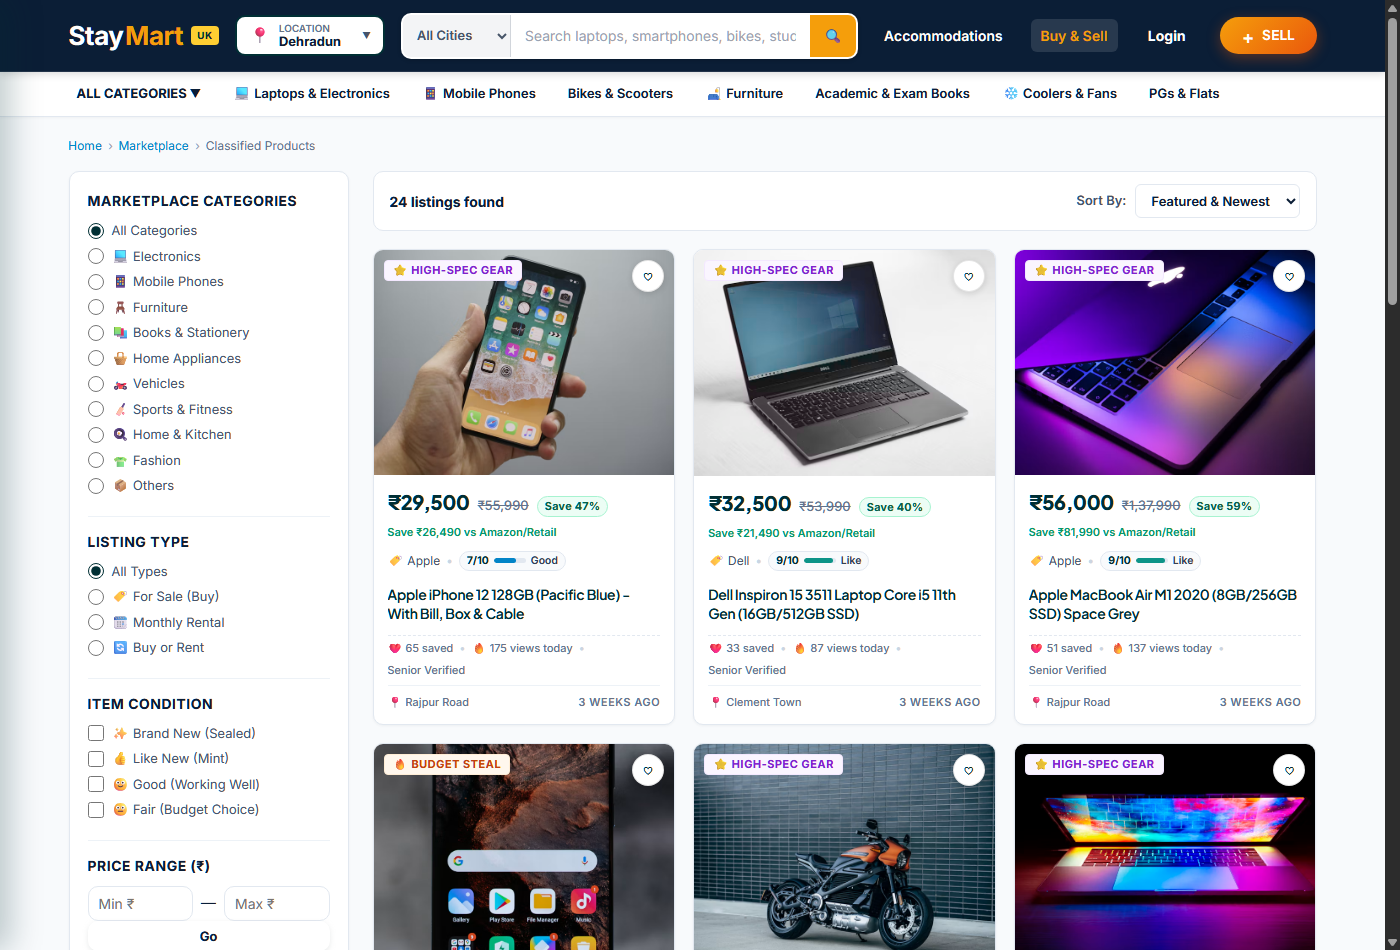
\includegraphics[width=\textwidth]{screenshots/search_products.png}
        \caption{Product Search with Category Filter}
    \end{subfigure}
    \caption{Faceted Search Interfaces with Real Listing Photography}
    \label{fig:search_screens}
\end{figure}

Features include: multi-variable filters (city, zone, budget, sharing type, amenities), standardized 4:3 image cards, and slide-up mobile filter drawers with zero horizontal overflow.

\subsection{Listing Detail Portals}
Detail views (\texttt{property-detail.html} and \texttt{product-detail.html}) present verified specifications, photo galleries, landlord contacts, and room reservation widgets (Figure \ref{fig:detail_screens}).

\begin{figure}[htbp]
    \centering
    \begin{subfigure}[b]{0.48\textwidth}
        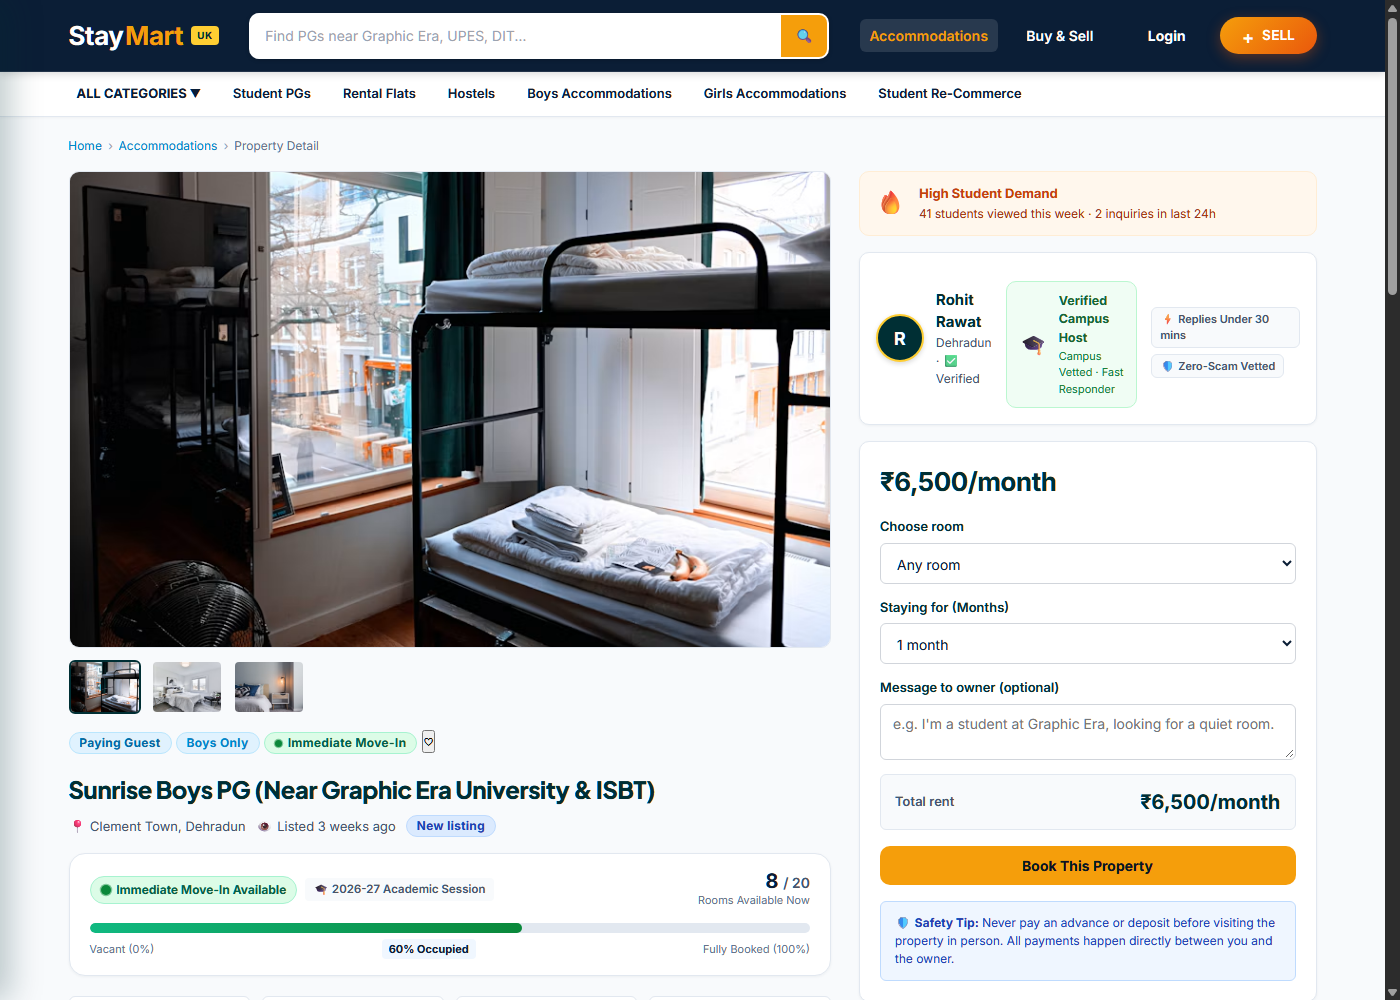
\includegraphics[width=\textwidth]{screenshots/property_detail.png}
        \caption{Property Details and Room Booking Widget}
    \end{subfigure}
    \hfill
    \begin{subfigure}[b]{0.48\textwidth}
        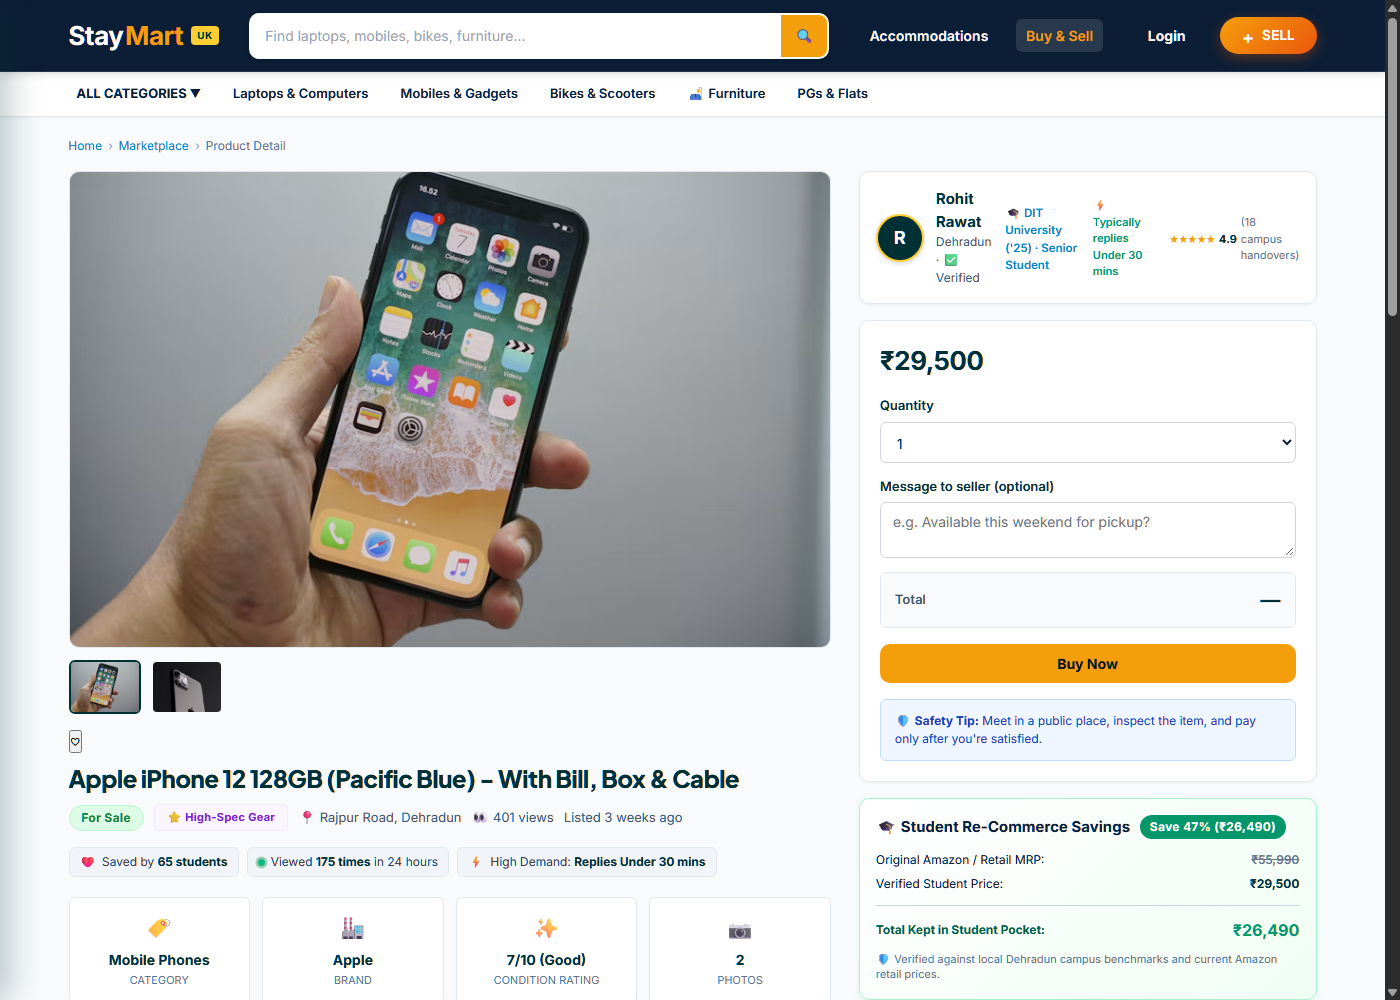
\includegraphics[width=\textwidth]{screenshots/product_detail.png}
        \caption{Product Details with Specifications}
    \end{subfigure}
    \caption{Listing Detail Pages with Interactive Galleries and Host Details}
    \label{fig:detail_screens}
\end{figure}

\subsection{Listing Submission and Publishing Portals}
Registered hosts and students publish listings through structured self-service forms (\texttt{post-property.html} and \texttt{post-product.html}) guiding inventory creation (Figure \ref{fig:post_screens}).

\begin{figure}[htbp]
    \centering
    \begin{subfigure}[b]{0.48\textwidth}
        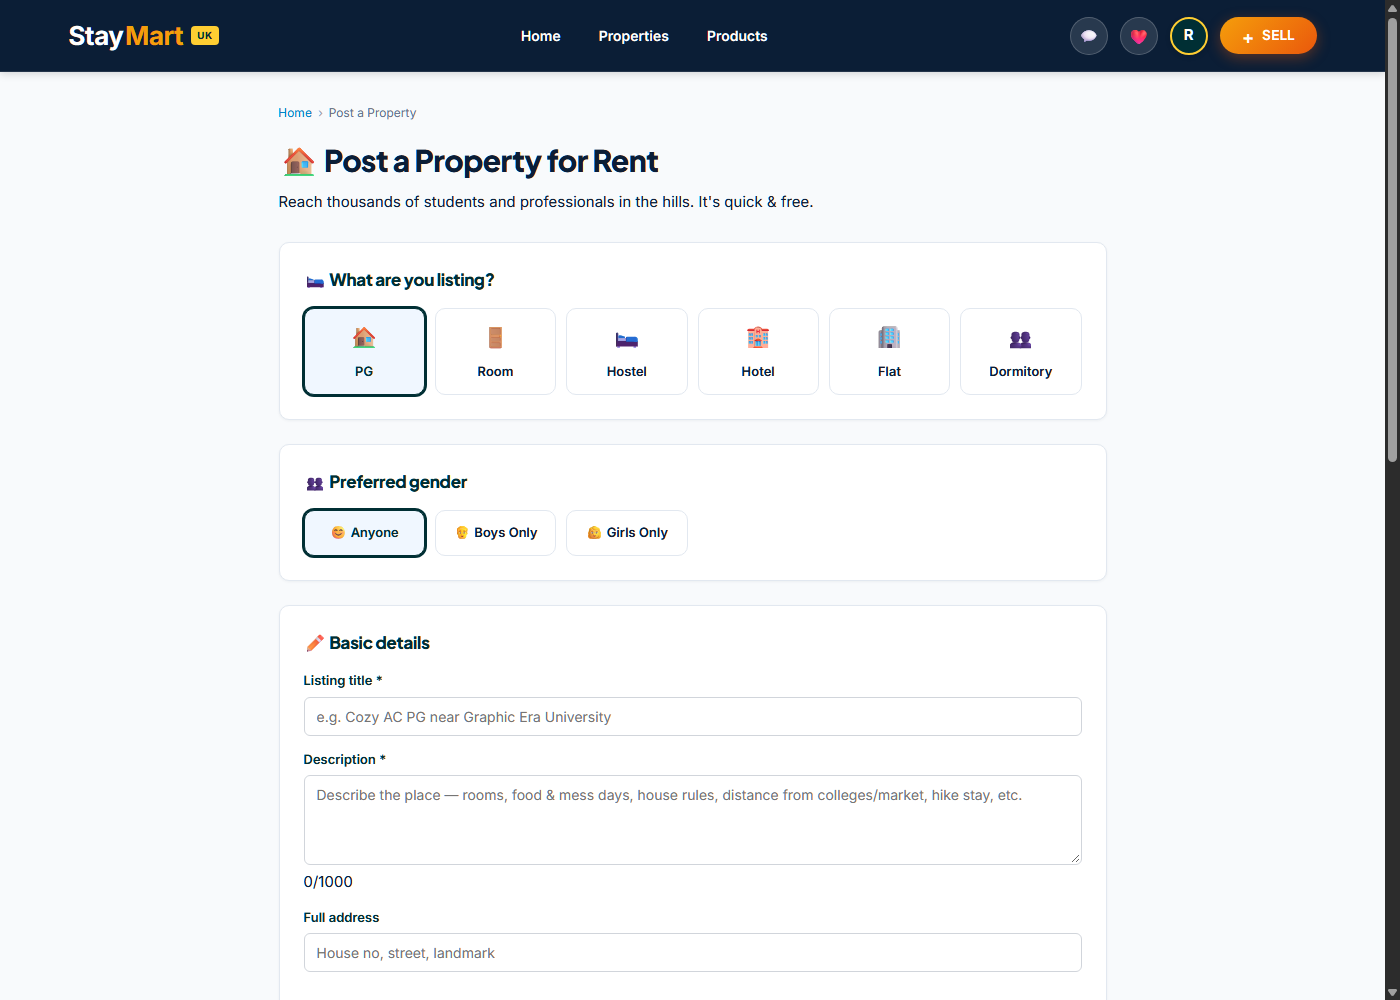
\includegraphics[width=\textwidth]{screenshots/post_property.png}
        \caption{Accommodation Listing Submission Form}
    \end{subfigure}
    \hfill
    \begin{subfigure}[b]{0.48\textwidth}
        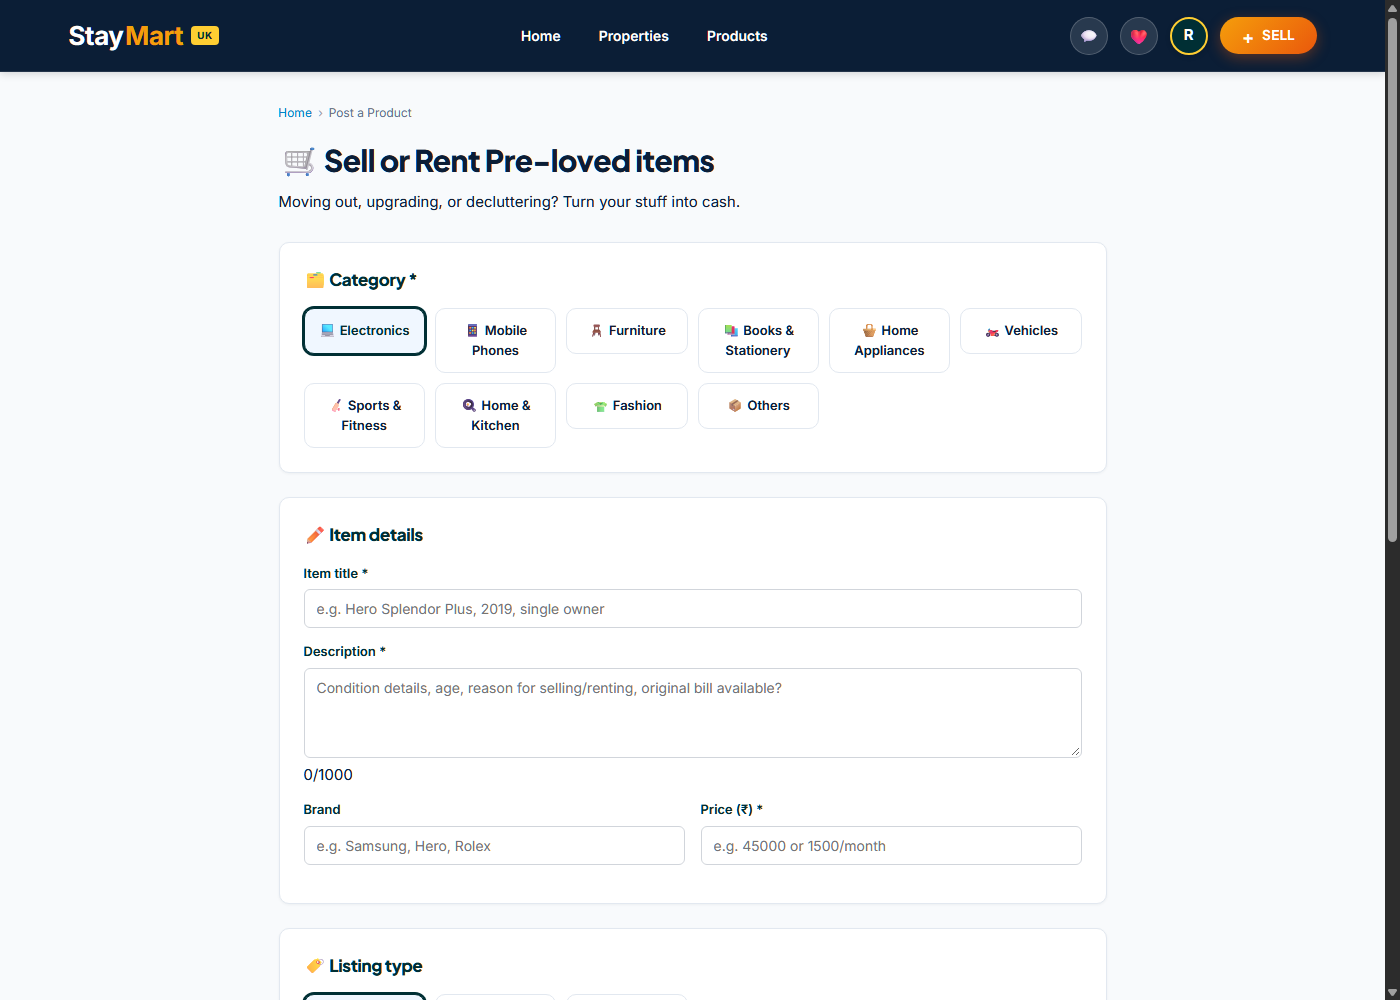
\includegraphics[width=\textwidth]{screenshots/post_product.png}
        \caption{Student Re-Commerce Product Form}
    \end{subfigure}
    \caption{Self-Service Listing Creation Portals for Accommodations and Student Marketplace}
    \label{fig:post_screens}
\end{figure}

\section{Self-Service User and Admin Management Portals}

\subsection{User Dashboard and Peer Messaging Portals}
The user dashboard (\texttt{pages/user/dashboard.html}) and messaging center (\texttt{pages/user/chat.html}) consolidate personal interactions (Figure \ref{fig:user_portal_screens}).

\begin{figure}[htbp]
    \centering
    \begin{subfigure}[b]{0.48\textwidth}
        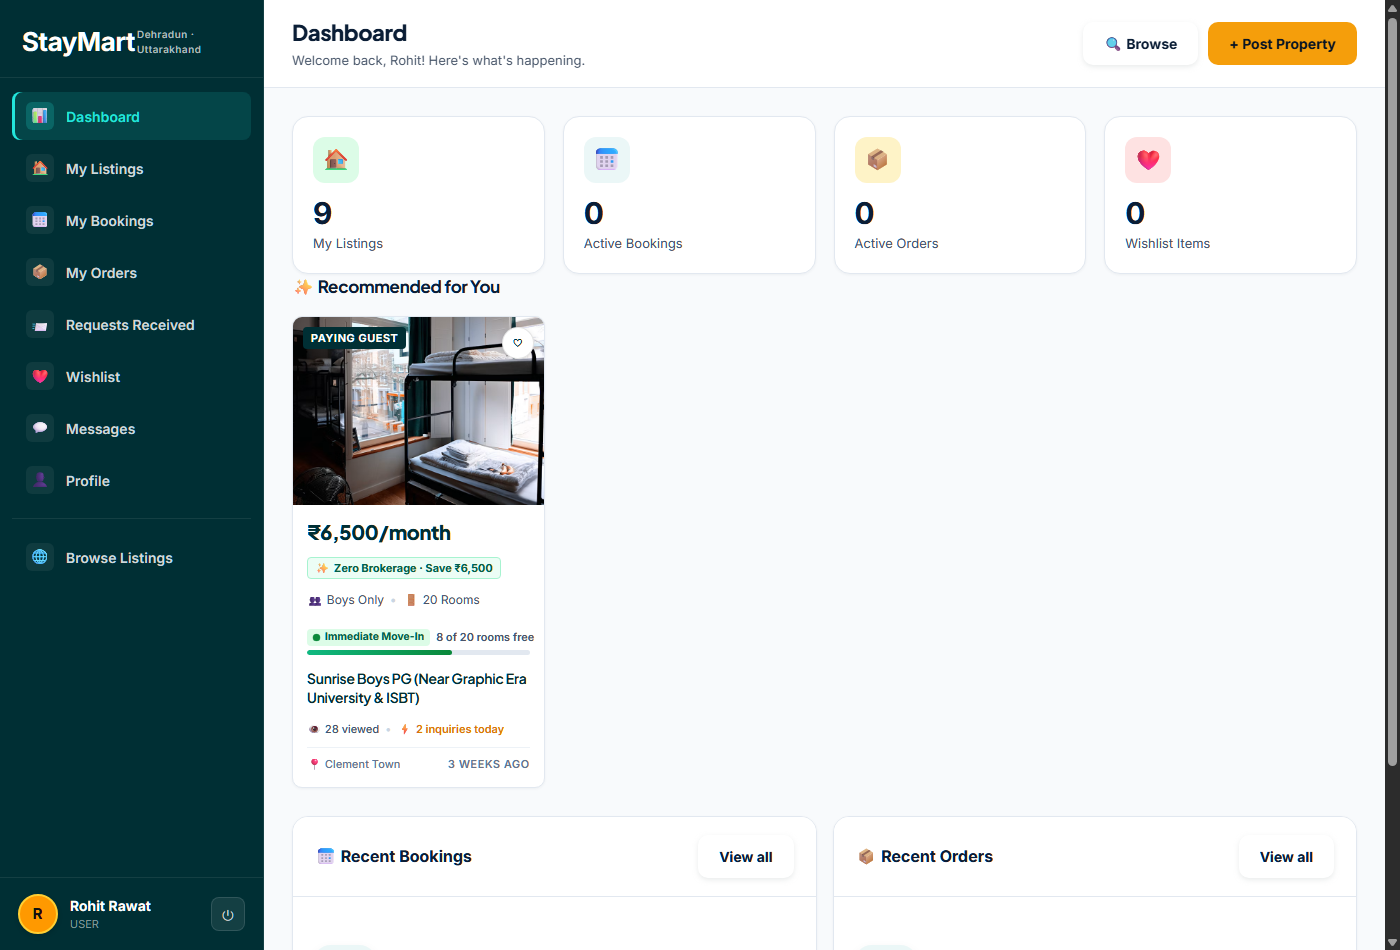
\includegraphics[width=\textwidth]{screenshots/user_dashboard.png}
        \caption{User Activity Dashboard and Recommendations}
    \end{subfigure}
    \hfill
    \begin{subfigure}[b]{0.48\textwidth}
        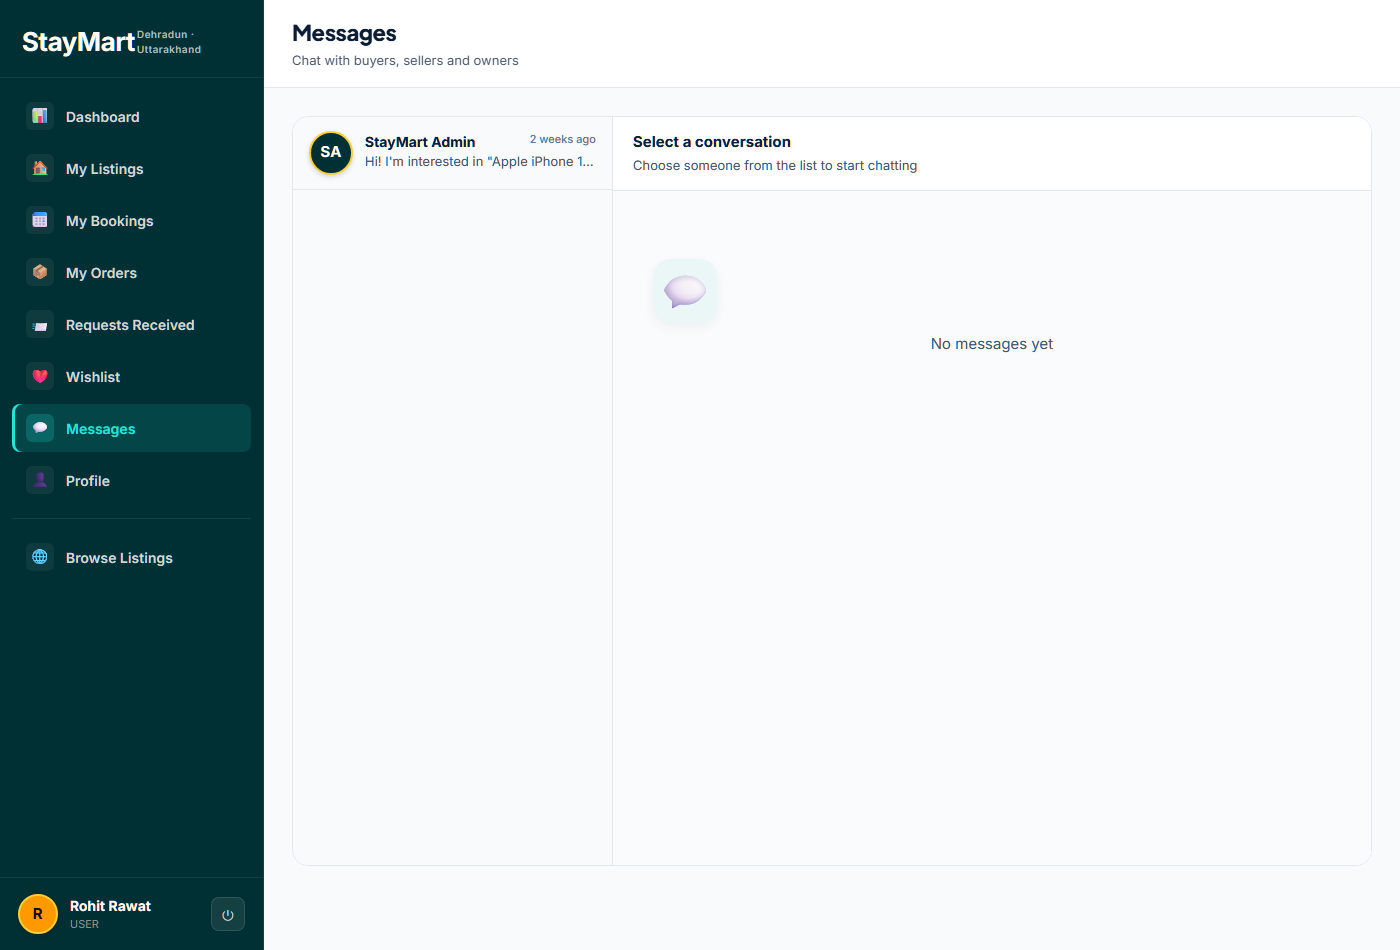
\includegraphics[width=\textwidth]{screenshots/user_chat.png}
        \caption{In-App Peer Chat with Caretaker}
    \end{subfigure}
    \caption{Self-Service User Dashboard and Real-Time Peer Messaging Interfaces}
    \label{fig:user_portal_screens}
\end{figure}

\subsection{Administrative Moderation and Governance Console}
Platform staff govern listings and users through \texttt{pages/admin/dashboard.html} (Figure \ref{fig:admin_dashboard_ui}).

\begin{figure}[htbp]
    \centering
    \begin{subfigure}[b]{0.48\textwidth}
        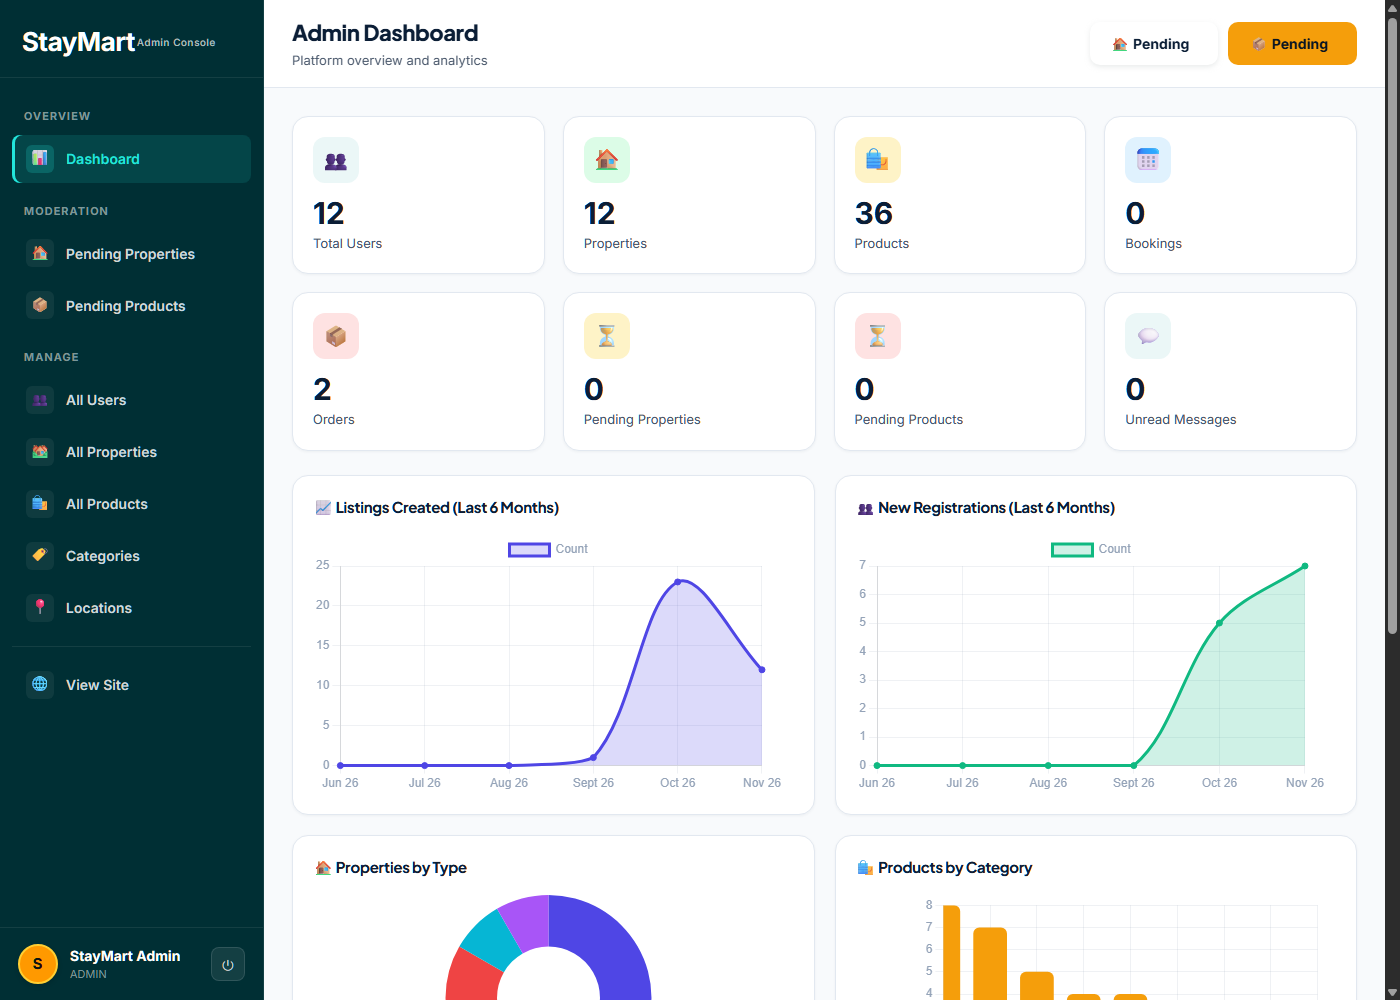
\includegraphics[width=\textwidth]{screenshots/admin_dashboard.png}
        \caption{Administrative Metrics Console}
    \end{subfigure}
    \hfill
    \begin{subfigure}[b]{0.48\textwidth}
        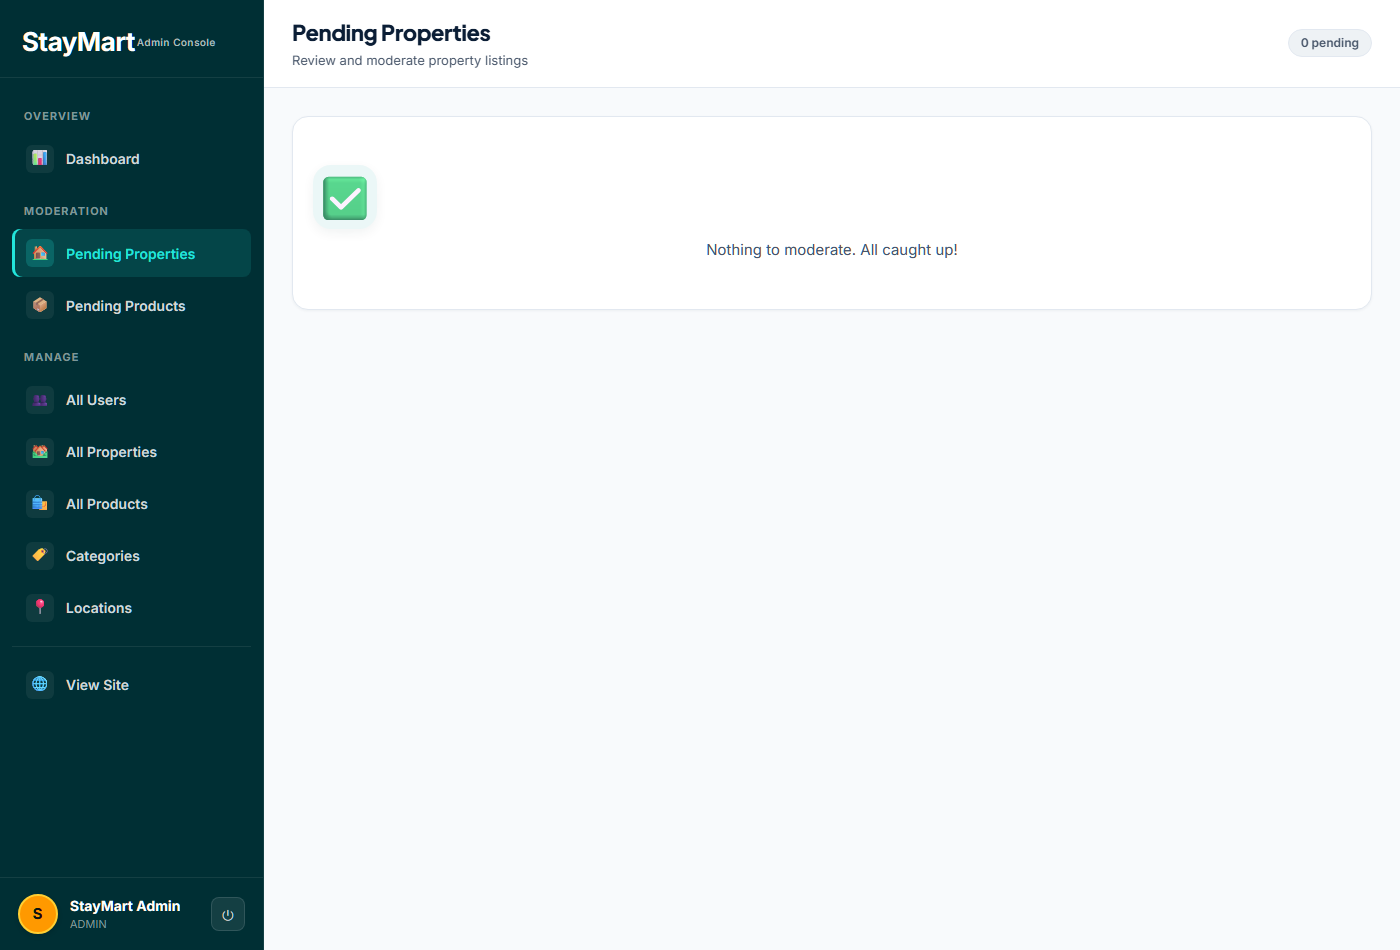
\includegraphics[width=\textwidth]{screenshots/admin_pending_properties.png}
        \caption{Listing Moderation Approval Queue}
    \end{subfigure}
    \caption{Administrative Console Featuring Live Platform Metrics and Pre-Publication Moderation Queue}
    \label{fig:admin_dashboard_ui}
\end{figure}

\section{Summary}
This chapter detailed StayMart's commercial light design system, design tokens, modular ES6 JavaScript architecture, and responsive user flows across accommodations, re-commerce, and admin moderation. The following chapter presents verification, testing results, and system walkthroughs.
